\section{Desktop/cleanstuff/i-team/trunk/iteam\_\-maths.cpp File Reference}
\label{iteam__maths_8cpp}\index{Desktop/cleanstuff/i-team/trunk/iteam_maths.cpp@{Desktop/cleanstuff/i-team/trunk/iteam\_\-maths.cpp}}
Mathematical functions. 

{\tt \#include \char`\"{}iteam\_\-maths.h\char`\"{}}\par
{\tt \#include $<$iostream$>$}\par
{\tt \#include $<$cmath$>$}\par


Include dependency graph for iteam\_\-maths.cpp:\nopagebreak
\begin{figure}[H]
\begin{center}
\leavevmode
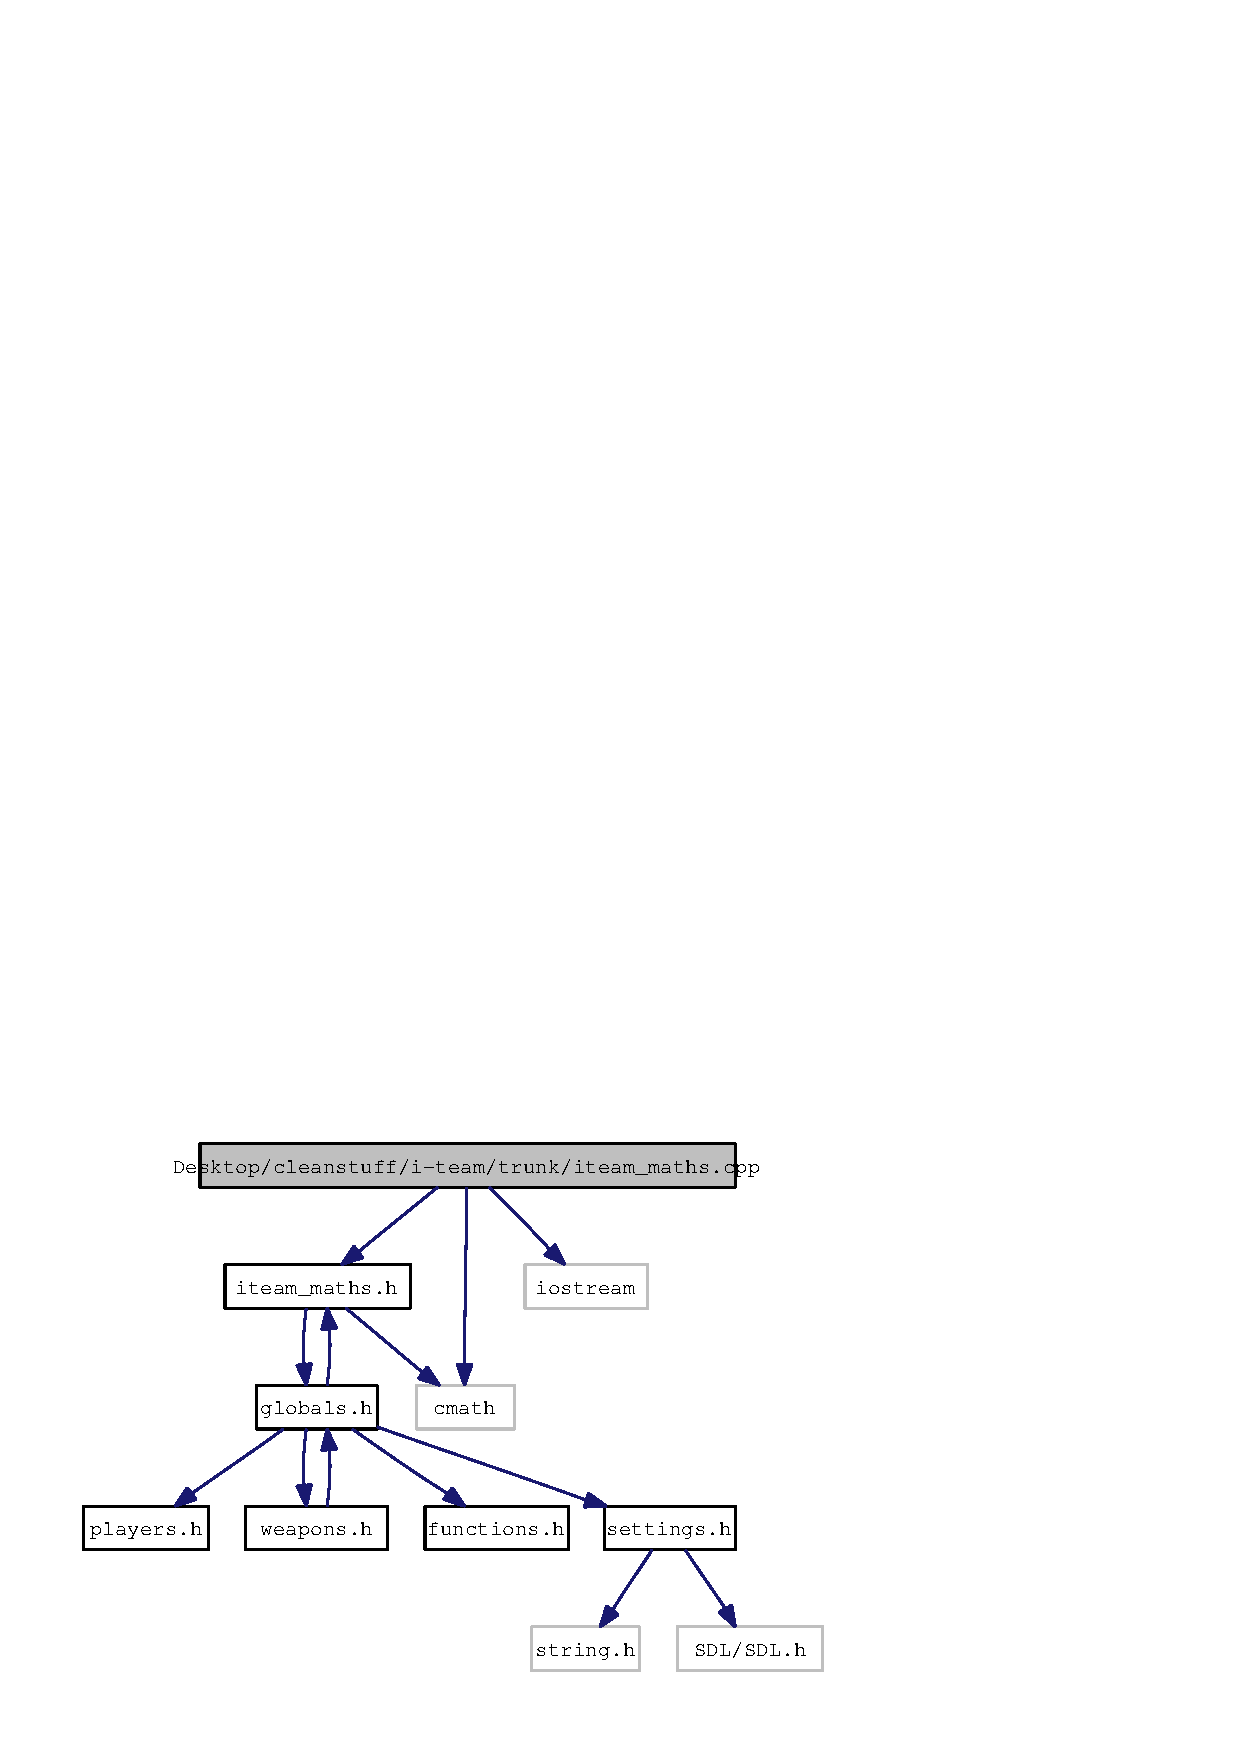
\includegraphics[width=199pt]{iteam__maths_8cpp__incl}
\end{center}
\end{figure}
\subsection*{Functions}
\begin{CompactItemize}
\item 
GLfloat {\bf deg2rad} (GLfloat a\_\-deg)\label{iteam__maths_8cpp_3058d94a2d148c090c62712dd1a0a215}

\begin{CompactList}\small\item\em Converts degrees to radians. \item\end{CompactList}\item 
GLfloat {\bf rad2deg} (GLfloat a\_\-rad)\label{iteam__maths_8cpp_b95d84f6a14b4237d444c97611da6bea}

\begin{CompactList}\small\item\em Converts radians to degrees. \item\end{CompactList}\item 
GLfloat {\bf limit\_\-angle} (GLfloat angle)\label{iteam__maths_8cpp_fba60a0485018bb94efdde2c82906285}

\begin{CompactList}\small\item\em Makes sure the angle stays in [0;360[. \item\end{CompactList}\item 
void {\bf init\_\-rand} ()\label{iteam__maths_8cpp_ce6a4b0f49666a9bc4b4b1bee884d480}

\begin{CompactList}\small\item\em Initialize random seed. \item\end{CompactList}\item 
GLfloat {\bf rand\_\-uniform} (GLfloat min, GLfloat max)\label{iteam__maths_8cpp_09ad0f4f0bd2d75bca4401a28bb5e2a8}

\begin{CompactList}\small\item\em Returns a random number between min and max using a uniform distribution. Originally created to add an error to the shots calculated by the AI. \item\end{CompactList}\item 
int {\bf T\_\-reflect\_\-vector} (double Tx, double Ty, double Vx, double Vy, GLfloat \&Vpx, GLfloat \&Vpy)\label{iteam__maths_8cpp_4fe21ddfcb8e616e08adcb1bfd42e718}

\begin{CompactList}\small\item\em Calculates the \char`\"{}reflection\char`\"{} vec(Vp) of the velocity vector vec(V) on the slope vec(T). Returns 0 if vec(T)=0. \item\end{CompactList}\item 
int {\bf N\_\-reflect\_\-vector} (double Nx, double Ny, double Vx, double Vy, GLfloat \&Vpx, GLfloat \&Vpy)\label{iteam__maths_8cpp_46394c0acfe63de175107fb648ec74e8}

\begin{CompactList}\small\item\em Calculates the \char`\"{}reflection\char`\"{} vec(Vp) of the velocity vector vec(V) on the normal vec(N). Returns 0 if vec(N)=0. \item\end{CompactList}\item 
GLfloat {\bf DistanceBetween} (GLfloat x1, GLfloat y1, GLfloat x2, GLfloat y2)\label{iteam__maths_8cpp_7212744857924b223ed1f60b162b20e0}

\begin{CompactList}\small\item\em Returns the distance between two 2d points (x1,y1) and (x2,y2). \item\end{CompactList}\item 
GLfloat {\bf AngleBetweenObjects} (GLfloat x1, GLfloat y1, GLfloat x2, GLfloat y2)\label{iteam__maths_8cpp_c4f8d649072c19292317794a3f874ba2}

\begin{CompactList}\small\item\em Returns the angle between two 2d vectors (x1,y1) and (x2,y2). \item\end{CompactList}\end{CompactItemize}


\subsection{Detailed Description}
Mathematical functions. 

various maths \& pysics functions 